\documentclass[ignorenonframetext,]{beamer}
\setbeamertemplate{caption}[numbered]
\setbeamertemplate{caption label separator}{: }
\setbeamercolor{caption name}{fg=normal text.fg}
\beamertemplatenavigationsymbolsempty
\usepackage{lmodern}
\usepackage{amssymb,amsmath}
\usepackage{ifxetex,ifluatex}
\usepackage{fixltx2e} % provides \textsubscript
\ifnum 0\ifxetex 1\fi\ifluatex 1\fi=0 % if pdftex
  \usepackage[T1]{fontenc}
  \usepackage[utf8]{inputenc}
\else % if luatex or xelatex
  \ifxetex
    \usepackage{mathspec}
  \else
    \usepackage{fontspec}
  \fi
  \defaultfontfeatures{Ligatures=TeX,Scale=MatchLowercase}
\fi
\usetheme[]{Madrid}
\usecolortheme{crane}
\usefonttheme{professionalfonts}
% use upquote if available, for straight quotes in verbatim environments
\IfFileExists{upquote.sty}{\usepackage{upquote}}{}
% use microtype if available
\IfFileExists{microtype.sty}{%
\usepackage{microtype}
\UseMicrotypeSet[protrusion]{basicmath} % disable protrusion for tt fonts
}{}
\newif\ifbibliography
\hypersetup{
            pdftitle={Introduction to R},
            pdfborder={0 0 0},
            breaklinks=true}
\urlstyle{same}  % don't use monospace font for urls
\usepackage{color}
\usepackage{fancyvrb}
\newcommand{\VerbBar}{|}
\newcommand{\VERB}{\Verb[commandchars=\\\{\}]}
\DefineVerbatimEnvironment{Highlighting}{Verbatim}{commandchars=\\\{\}}
% Add ',fontsize=\small' for more characters per line
\usepackage{framed}
\definecolor{shadecolor}{RGB}{248,248,248}
\newenvironment{Shaded}{\begin{snugshade}}{\end{snugshade}}
\newcommand{\KeywordTok}[1]{\textcolor[rgb]{0.13,0.29,0.53}{\textbf{#1}}}
\newcommand{\DataTypeTok}[1]{\textcolor[rgb]{0.13,0.29,0.53}{#1}}
\newcommand{\DecValTok}[1]{\textcolor[rgb]{0.00,0.00,0.81}{#1}}
\newcommand{\BaseNTok}[1]{\textcolor[rgb]{0.00,0.00,0.81}{#1}}
\newcommand{\FloatTok}[1]{\textcolor[rgb]{0.00,0.00,0.81}{#1}}
\newcommand{\ConstantTok}[1]{\textcolor[rgb]{0.00,0.00,0.00}{#1}}
\newcommand{\CharTok}[1]{\textcolor[rgb]{0.31,0.60,0.02}{#1}}
\newcommand{\SpecialCharTok}[1]{\textcolor[rgb]{0.00,0.00,0.00}{#1}}
\newcommand{\StringTok}[1]{\textcolor[rgb]{0.31,0.60,0.02}{#1}}
\newcommand{\VerbatimStringTok}[1]{\textcolor[rgb]{0.31,0.60,0.02}{#1}}
\newcommand{\SpecialStringTok}[1]{\textcolor[rgb]{0.31,0.60,0.02}{#1}}
\newcommand{\ImportTok}[1]{#1}
\newcommand{\CommentTok}[1]{\textcolor[rgb]{0.56,0.35,0.01}{\textit{#1}}}
\newcommand{\DocumentationTok}[1]{\textcolor[rgb]{0.56,0.35,0.01}{\textbf{\textit{#1}}}}
\newcommand{\AnnotationTok}[1]{\textcolor[rgb]{0.56,0.35,0.01}{\textbf{\textit{#1}}}}
\newcommand{\CommentVarTok}[1]{\textcolor[rgb]{0.56,0.35,0.01}{\textbf{\textit{#1}}}}
\newcommand{\OtherTok}[1]{\textcolor[rgb]{0.56,0.35,0.01}{#1}}
\newcommand{\FunctionTok}[1]{\textcolor[rgb]{0.00,0.00,0.00}{#1}}
\newcommand{\VariableTok}[1]{\textcolor[rgb]{0.00,0.00,0.00}{#1}}
\newcommand{\ControlFlowTok}[1]{\textcolor[rgb]{0.13,0.29,0.53}{\textbf{#1}}}
\newcommand{\OperatorTok}[1]{\textcolor[rgb]{0.81,0.36,0.00}{\textbf{#1}}}
\newcommand{\BuiltInTok}[1]{#1}
\newcommand{\ExtensionTok}[1]{#1}
\newcommand{\PreprocessorTok}[1]{\textcolor[rgb]{0.56,0.35,0.01}{\textit{#1}}}
\newcommand{\AttributeTok}[1]{\textcolor[rgb]{0.77,0.63,0.00}{#1}}
\newcommand{\RegionMarkerTok}[1]{#1}
\newcommand{\InformationTok}[1]{\textcolor[rgb]{0.56,0.35,0.01}{\textbf{\textit{#1}}}}
\newcommand{\WarningTok}[1]{\textcolor[rgb]{0.56,0.35,0.01}{\textbf{\textit{#1}}}}
\newcommand{\AlertTok}[1]{\textcolor[rgb]{0.94,0.16,0.16}{#1}}
\newcommand{\ErrorTok}[1]{\textcolor[rgb]{0.64,0.00,0.00}{\textbf{#1}}}
\newcommand{\NormalTok}[1]{#1}
\usepackage{longtable,booktabs}
\usepackage{caption}
% These lines are needed to make table captions work with longtable:
\makeatletter
\def\fnum@table{\tablename~\thetable}
\makeatother
\usepackage{graphicx,grffile}
\makeatletter
\def\maxwidth{\ifdim\Gin@nat@width>\linewidth\linewidth\else\Gin@nat@width\fi}
\def\maxheight{\ifdim\Gin@nat@height>\textheight0.8\textheight\else\Gin@nat@height\fi}
\makeatother
% Scale images if necessary, so that they will not overflow the page
% margins by default, and it is still possible to overwrite the defaults
% using explicit options in \includegraphics[width, height, ...]{}
\setkeys{Gin}{width=\maxwidth,height=\maxheight,keepaspectratio}

% Prevent slide breaks in the middle of a paragraph:
\widowpenalties 1 10000
\raggedbottom

\AtBeginPart{
  \let\insertpartnumber\relax
  \let\partname\relax
  \frame{\partpage}
}
\AtBeginSection{
  \ifbibliography
  \else
    \let\insertsectionnumber\relax
    \let\sectionname\relax
    \frame{\sectionpage}
  \fi
}
\AtBeginSubsection{
  \let\insertsubsectionnumber\relax
  \let\subsectionname\relax
  \frame{\subsectionpage}
}

\setlength{\parindent}{0pt}
\setlength{\parskip}{6pt plus 2pt minus 1pt}
\setlength{\emergencystretch}{3em}  % prevent overfull lines
\providecommand{\tightlist}{%
  \setlength{\itemsep}{0pt}\setlength{\parskip}{0pt}}
\setcounter{secnumdepth}{0}
\usepackage{booktabs}
\usepackage{hyperref}
\usepackage{caption}
\usepackage{graphicx}
\usepackage{amsmath}
\usepackage{graphics}
\author[SCC]{Statistical Consulting Centre}
\institute[\href{mailto:consulting@stat.auckland.ac.nz}
			{consulting@stat.auckland.ac.nz}]{\href{mailto:consulting@stat.auckland.ac.nz}
			{consulting@stat.auckland.ac.nz}\\
			The Department of Statistics\\
			The University of Auckland}
\titlegraphic{
\includegraphics[width=5cm]{..//..//S-DS-VC-RGB.png}}
\let\oldShaded\Shaded
\let\endoldShaded\endShaded
\renewenvironment{Shaded}{\footnotesize\oldShaded}{\endoldShaded}
\let\oldverbatim\verbatim
\let\endoldverbatim\endverbatim
\renewenvironment{verbatim}{\footnotesize\oldverbatim}{\endoldverbatim}

\title{Introduction to \textbf{R}}
\subtitle{Session 1 -- Introduction}
\date{9-10 July 2018}

\begin{document}
\frame{\titlepage}

\begin{frame}{Monday}

Each session comprises two parts: lecture and practice.

\begin{longtable}[]{@{}lll@{}}
\toprule
Session & Time & Topic\tabularnewline
\midrule
\endhead
1 & 09:00am - 10:30am & Introduction and Data Import\tabularnewline
& 10:30am - 11:00am & Break\tabularnewline
2 & 11:00am - 12:30pm & Descriptive statistics\tabularnewline
& 12:30pm - 01:30pm & Lunch break\tabularnewline
3 & 01:30pm - 03:00pm & Basic R programming\tabularnewline
& 03:00pm - 03:30pm & Break\tabularnewline
4 & 03:30pm - 05:00pm & Advanced R programming\tabularnewline
\bottomrule
\end{longtable}

\end{frame}

\begin{frame}{Tuesday}

Each session comprises two parts: lecture and practice.

\begin{longtable}[]{@{}lll@{}}
\toprule
Session & Time & Topic\tabularnewline
\midrule
\endhead
1 & 09:00am - 10:30am & Graphics\tabularnewline
& 10:30am - 11:00am & Break\tabularnewline
2 & 11:00am - 12:30pm & Advanced Graphics (ggplot2)\tabularnewline
& 12:30pm - 01:30pm & Lunch break\tabularnewline
3 & 01:30pm - 03:00pm & Basic analysis\tabularnewline
& 03:00pm - 03:30pm & Break\tabularnewline
4 & 03:30pm - 05:00pm & Advanced analysis (R Markdown)\tabularnewline
\bottomrule
\end{longtable}

\end{frame}

\begin{frame}{What is \textbf{R}?}

\begin{quote}
\textbf{R} is a free software environment for statistical computing and
graphics
\end{quote}

\begin{itemize}
\tightlist
\item
  Created by Ross Ihaka and Robert Gentleman of the Department of
  Statistics, University of Auckland.
\item
  First version was made available in 1995.
\item
  Has become one of the most popular environments for statistical
  computing and data science.
\item
  We have three members of the \emph{\textbf{R} Development Core Team}
  in the Department of Statistics.
\end{itemize}

\center 
\includegraphics[width=5.00000cm]{..//..//S-DS-VC-RGB.png}

\end{frame}

\begin{frame}{Why is \textbf{R} so popular?}

\begin{itemize}
\item
  It is open-source (FREE)!
\item
  It is powerful:

  \begin{itemize}
  \tightlist
  \item
    Can handle large and complex data sets.
  \item
    Easily program complex simulations.
  \item
    Can be used on High-Performance Computing Cluster.
  \item
    Graphics (much more flexible than SAS, SPSS, JMP, etc.)
  \end{itemize}
\item
  Well-support (Stack Overflow, R-Bloggers) from communities of
  different fields, i.e. \textbf{R} packages.
  \url{https://cran.r-project.org/web/views/}.
\item
  It is flexible (your problem can likely be handled in \textbf{R}).
\item
  It runs well on many operating systems (Windows, Mac, and Linux).
\end{itemize}

\centering You don't need to be a programmer to use \textbf{R}!

\end{frame}

\begin{frame}[fragile]{\textbf{R} and the biological sciences}

\begin{itemize}
\item
  Many applications of statistical methods to biological datasets are
  implemented in \textbf{R}.
\item
  These \textbf{R} \emph{packages} are publically available on the web
  for immediate download and use:

  \begin{itemize}
  \tightlist
  \item
    \texttt{Bioconductor}, \url{https://www.bioconductor.org/}
  \item
    E.g. Next Generation Sequencing, Genomics.
  \end{itemize}
\end{itemize}

\centering You don't need to be a programmer to use \textbf{R}!

\end{frame}

\begin{frame}{What is \textbf{R}? (IEEE Spectrum's ranking 2017)}

\center 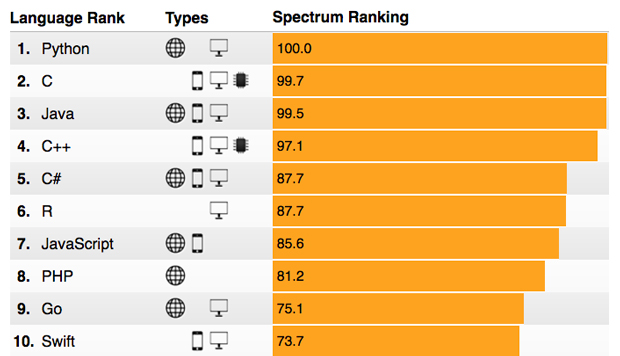
\includegraphics{Figure/ranking 2017.png}

\end{frame}

\begin{frame}{\textbf{R} and UoA's Department of Statistics}

\begin{quote}
If you want to learn \textbf{R}, you are talking to the right people!
\end{quote}

\center 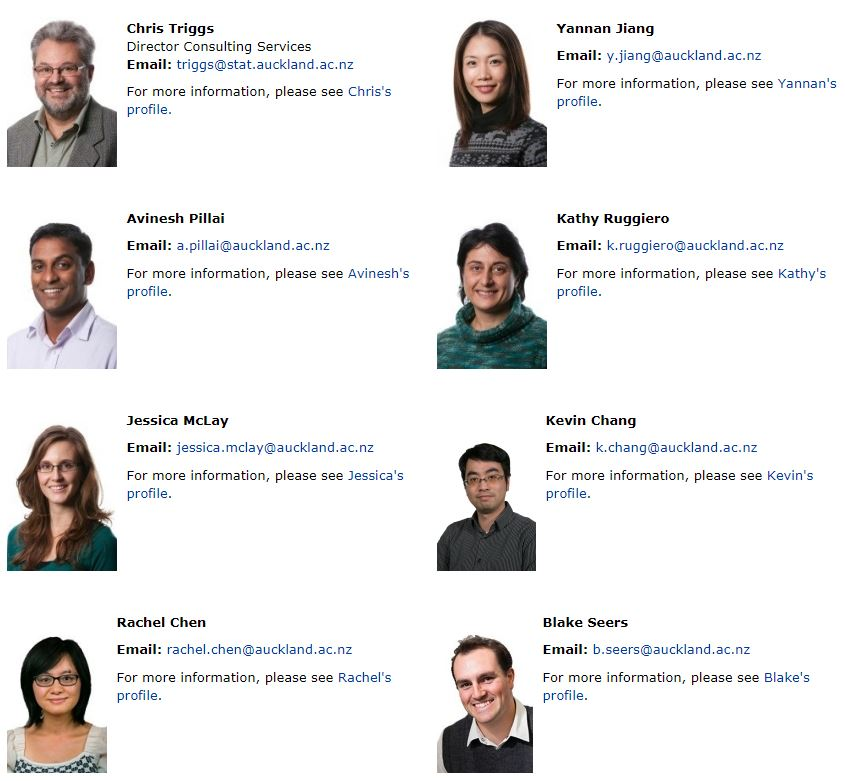
\includegraphics[width=2.60417in]{Figure/groupNew.jpg}

\end{frame}

\begin{frame}{Statistical Consulting Centre}

The School of Biological Sciences (SBS) has a contract with the
Statistical Consulting Centre to provide statistical support to staff
and postgraduate students of SBS.

\url{https://www.stat.auckland.ac.nz/consulting/meet-us/any1_uoa/appointment_scheduler_kevin}

\center 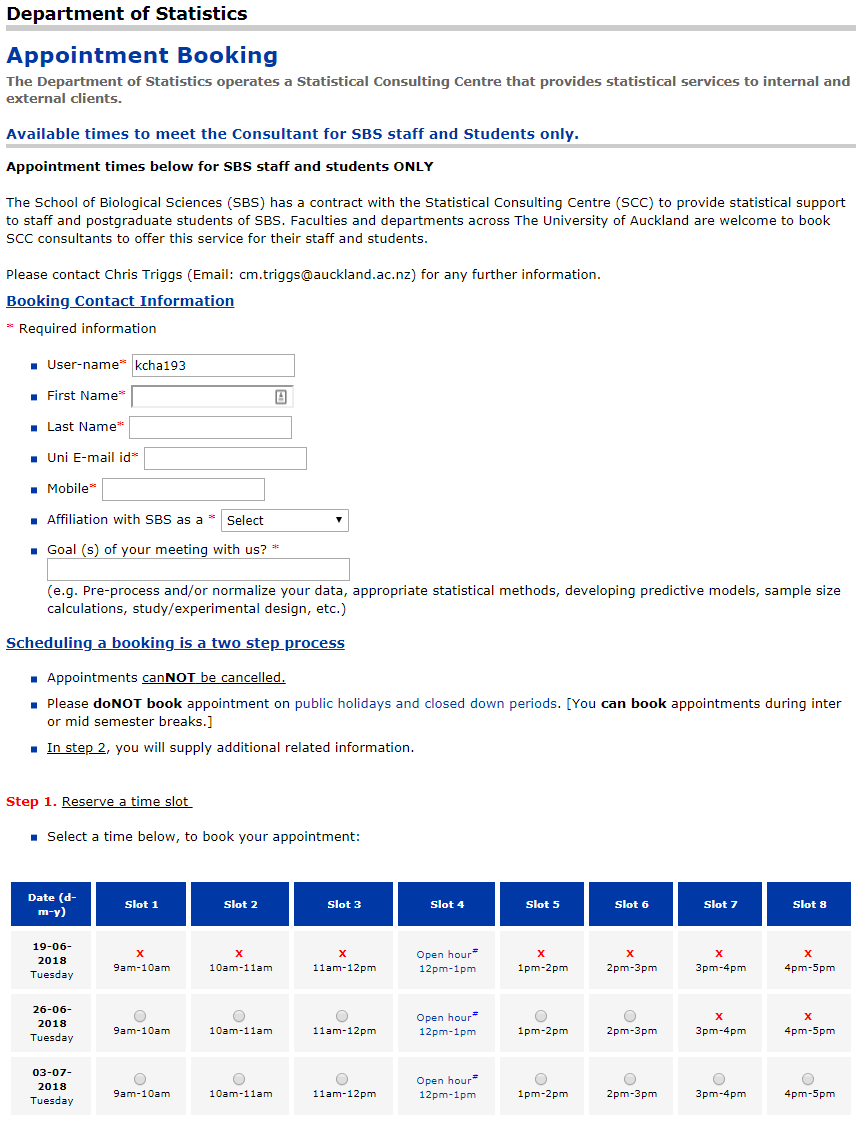
\includegraphics[width=2.60417in]{Figure/sbs booking.png}

\end{frame}

\begin{frame}{How to download and install \textbf{R} (and
\textbf{R}Studio)}

\begin{enumerate}
\def\labelenumi{\arabic{enumi}.}
\tightlist
\item
  Go to \url{https://cran.stat.auckland.ac.nz}.
\item
  Download the version relevant to your OS (Linux / Mac
  \href{https://medium.com/@GalarnykMichael/install-r-and-rstudio-on-mac-e911606ce4f4}{(link)}
  / Windows).
\item
  Install it on your computer.
\end{enumerate}

We \emph{strongly} recommend using the \textbf{R} editor called
\textbf{R}Studio.

\begin{itemize}
\tightlist
\item
  Download and install it from \url{https://www.rstudio.com/download}.
\item
  UOA: Both softwares can be installed in the \emph{Software Center}.
\item
  Great for beginners and advanced use\textbf{R}s!
\end{itemize}

\begin{block}{Reasons to use RStudio}

\begin{itemize}
\tightlist
\item
  Writing better code faster with \textbf{R}.
\item
  Producing reports (\textbf{R} markdown).
\item
  Producing interactive reports/tools (Shiny).
\item
  Developing \textbf{R} packages.
\end{itemize}

\end{block}

\end{frame}

\begin{frame}{\textbf{R}studio}

\begin{itemize}
\tightlist
\item
  Now open \textbf{R}studio
\end{itemize}

\center 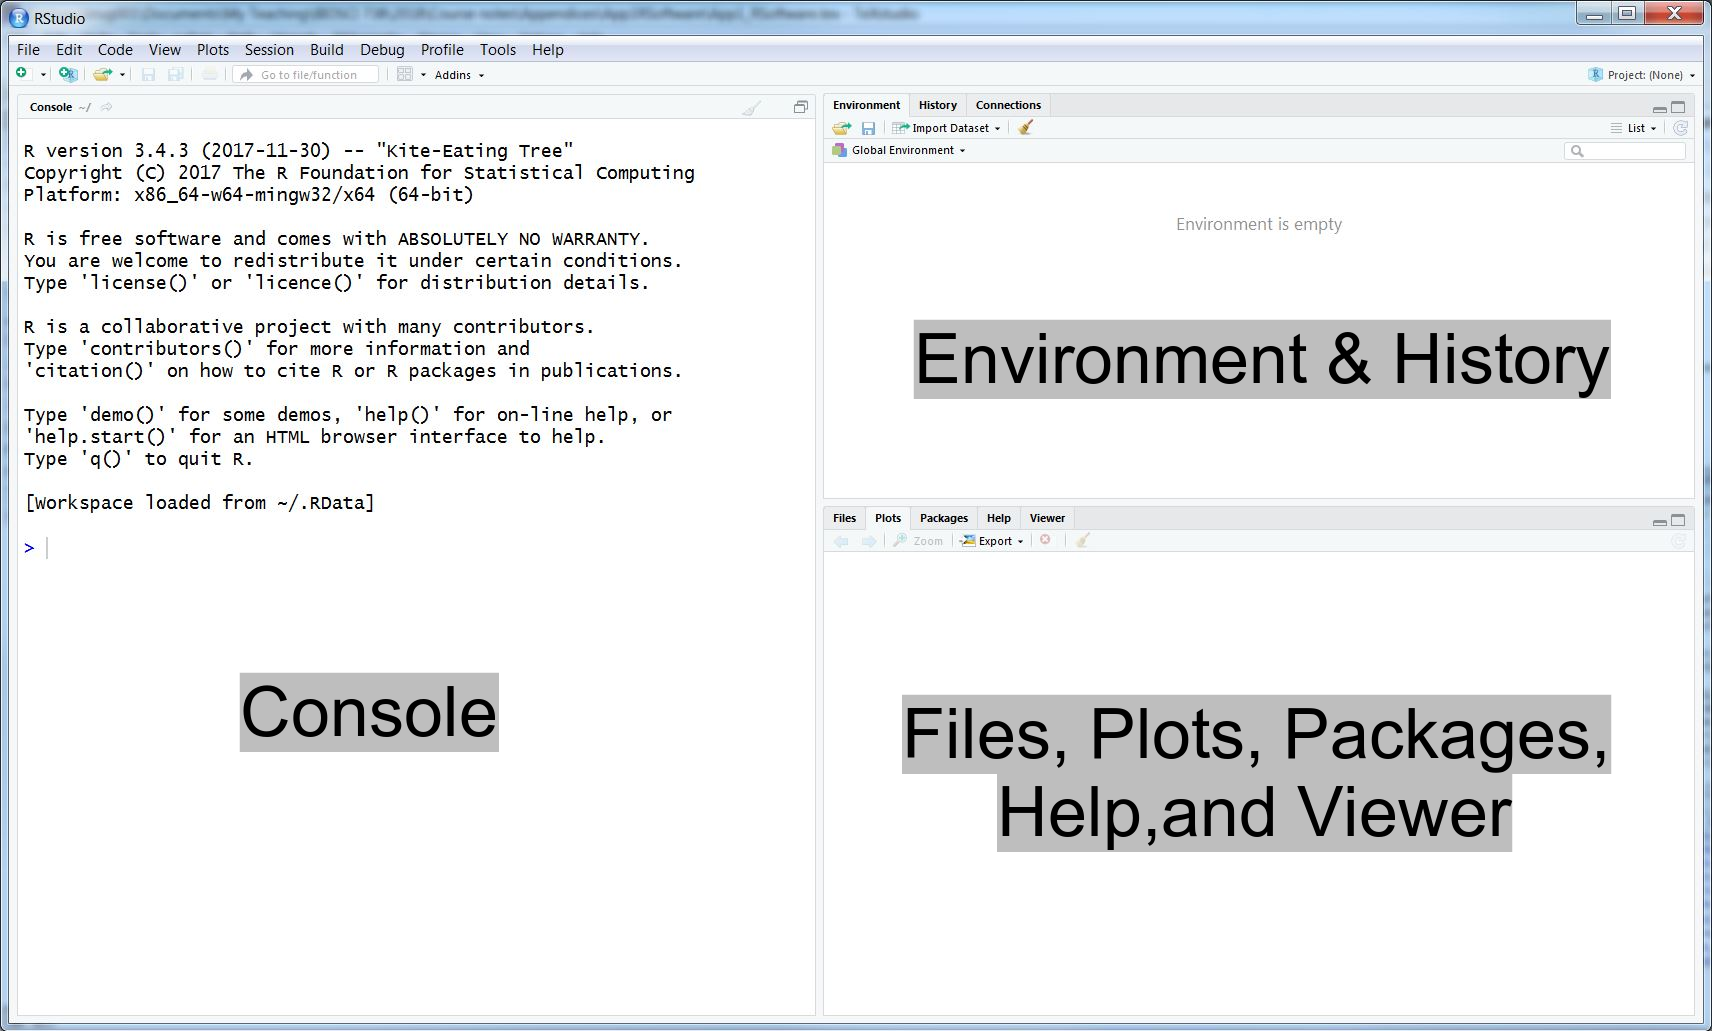
\includegraphics[width=8.00000cm]{Figure/rstudio.png}

\begin{itemize}
\tightlist
\item
  Then open an \textbf{R} script by clicking File \(\rightarrow\) New
  \(\rightarrow\) \textbf{R} script to show the \textbf{Source} pane.
\end{itemize}

\end{frame}

\begin{frame}{\textbf{R}studio Project}

\begin{itemize}
\item
  Divide your work into multiple contexts.
\item
  Each with their own

  \begin{itemize}
  \tightlist
  \item
    \textbf{working directory} (grey letters at the top of the Console),
  \item
    \textbf{workspace} (never save this),
  \item
    \textbf{history}, and
  \item
    \textbf{source documents} (\textbf{R} code).
  \end{itemize}
\item
  Cross-platform on different OS (Linux / Mac / Windows)
\end{itemize}

\begin{block}{Now create an \textbf{R}studio project for this workshop}

\begin{enumerate}
\def\labelenumi{\arabic{enumi}.}
\tightlist
\item
  Go to File \(\rightarrow\) ``New Project'',
\item
  Choose ``Existing directory'',
\item
  Click browse button to click \textbf{into} the folder ``Rwrkshop SBS
  2018'', and
\item
  Press ``open''.
\end{enumerate}

\end{block}

\end{frame}

\begin{frame}[fragile]{Using \textbf{R} as a calculator}

Again open an \textbf{R} script by clicking File \(\rightarrow\) New
\(\rightarrow\) \textbf{R} script and type and \textbf{run (Ctrl +
Enter)} the following in the \textbf{Source} pane.

\begin{Shaded}
\begin{Highlighting}[]
\DecValTok{1} \OperatorTok{+}\StringTok{ }\DecValTok{2}
\NormalTok{## [1] 3}

\DecValTok{1} \OperatorTok{+}\StringTok{ }\DecValTok{3}\OperatorTok{^}\DecValTok{2}
\NormalTok{## [1] 10}

\KeywordTok{log}\NormalTok{(}\DecValTok{15}\NormalTok{) }\OperatorTok{-}\StringTok{ }\KeywordTok{sqrt}\NormalTok{(}\FloatTok{3.4}\NormalTok{)}
\NormalTok{## [1] 0.8641413}

\KeywordTok{pnorm}\NormalTok{(}\FloatTok{1.96}\NormalTok{)}
\NormalTok{## [1] 0.9750021}

\CommentTok{# This is a comment and is not evaluated}
\end{Highlighting}
\end{Shaded}

\end{frame}

\begin{frame}[fragile]{Variable assignment}

\begin{itemize}
\tightlist
\item
  \texttt{\textless{}-} is the ``assign to'' operator, made up of
  \texttt{\textless{}} and \texttt{-} without a space.
\item
  E.g., \texttt{x\ \textless{}-\ 2} is read as ``The value 2 is assigned
  to the object \texttt{x}''.
\end{itemize}

\begin{Shaded}
\begin{Highlighting}[]
\NormalTok{x <-}\StringTok{ }\DecValTok{2}
\NormalTok{y <-}\StringTok{ }\DecValTok{3}
\NormalTok{x}\OperatorTok{^}\DecValTok{2} \OperatorTok{-}\StringTok{ }\DecValTok{3} \OperatorTok{*}\StringTok{ }\NormalTok{y }\OperatorTok{+}\StringTok{ }\DecValTok{5}
\NormalTok{## [1] 0}
\end{Highlighting}
\end{Shaded}

\begin{itemize}
\tightlist
\item
  You can also use \texttt{=} instead \texttt{\textless{}-}.
\end{itemize}

\begin{Shaded}
\begin{Highlighting}[]
\NormalTok{x =}\StringTok{ }\DecValTok{2}
\NormalTok{y =}\StringTok{ }\DecValTok{3}
\NormalTok{x}\OperatorTok{^}\DecValTok{2} \OperatorTok{-}\StringTok{ }\DecValTok{3} \OperatorTok{*}\StringTok{ }\NormalTok{y }\OperatorTok{+}\StringTok{ }\DecValTok{5}
\NormalTok{## [1] 0}
\end{Highlighting}
\end{Shaded}

Note that \textbf{R} is \textbf{case-sensitive}

\begin{Shaded}
\begin{Highlighting}[]
\NormalTok{X}
\NormalTok{## Error in eval(expr, envir, enclos): object 'X' not found}
\end{Highlighting}
\end{Shaded}

\end{frame}

\begin{frame}[fragile]{Getting help}

\begin{itemize}
\item
  Google!

  \begin{itemize}
  \tightlist
  \item
    ``How to calculate the average in \textbf{R}?''
  \item
    The search results tell you that the \texttt{mean()} function is
    useful.
  \end{itemize}
\item
  Quick-\textbf{R}: \url{https://www.statmethods.net/}
\item
  \textbf{R}-Bloggers: \url{https://www.r-bloggers.com/}
\item
  Stack Overflow: \url{https://stackoverflow.com/questions/tagged/r}
\item
  Books:

  \begin{itemize}
  \tightlist
  \item
    The \textbf{R} Book, by Michael J. Crawley.
  \item
    \textbf{R} for Data Science, by Hadley Wickham, Garrett Grolemund.
    \url{http://r4ds.had.co.nz/}
  \end{itemize}
\end{itemize}

\end{frame}

\begin{frame}[fragile]{Getting help -- in \textbf{R}}

\begin{itemize}
\item
  \texttt{?}

  For example, \texttt{?mean} brings up the help file for the
  \texttt{mean()} function. It will tell you almost everything you need
  to know to use \texttt{mean()}.
\item
  \texttt{??}

  For example, \texttt{??mean} searches for everything related to
  ``mean'' in all the \textbf{R} packages installed on your computer.
\item
  \texttt{RSiteSearch("mean")}

  Searches everything on CRAN (an online repository of \textbf{R}
  packages). This requires interenet connection.
\end{itemize}

\end{frame}

\begin{frame}{\textbf{R} documentation}

\center 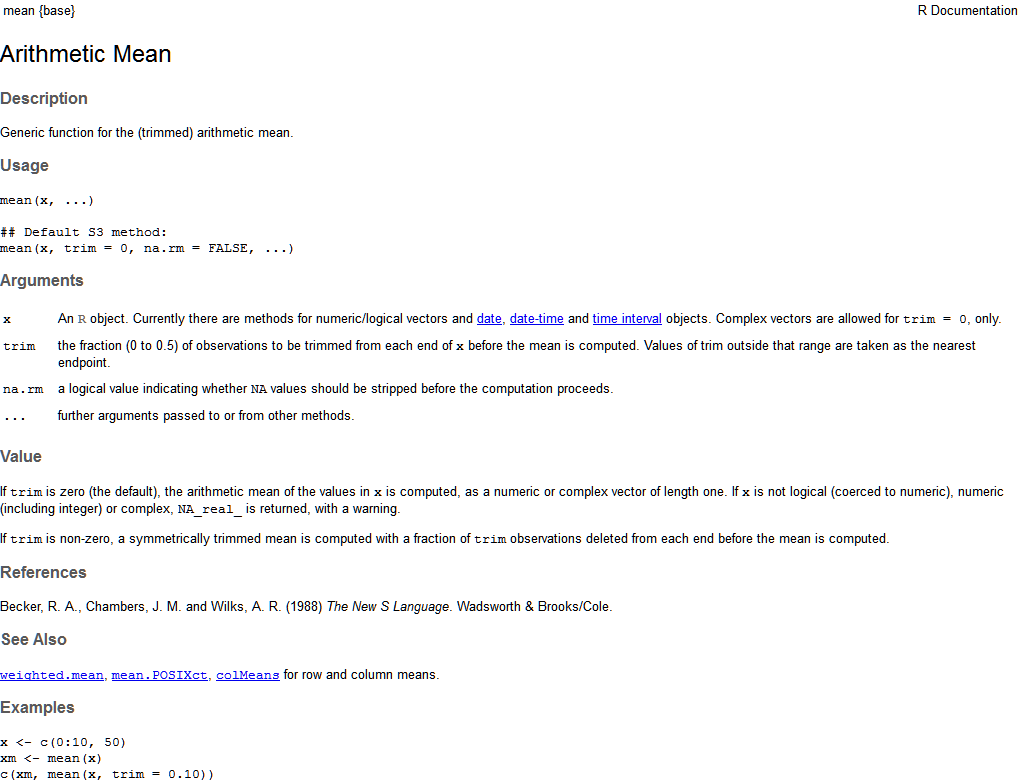
\includegraphics{Figure/mean function.png}

\end{frame}

\begin{frame}{Basic principles for data organisation in spreadsheets}

\begin{quote}
Whatever you do, do it consistently.
\end{quote}

Use consistent:

\begin{itemize}
\item
  codes for categorical variables (not M, Male, and male).
\item
  codes for missing values (can use NA or leave blank).

  \begin{itemize}
  \tightlist
  \item
    Do not use a numeric value (999).
  \end{itemize}
\item
  variable names in all files (glucose\_10wk, Gluc10wk)
\item
  subject identifiers (mouse153, M153, 153)
\item
  date formats (YYYY-MM-DD, YY/DD/MM)
\end{itemize}

Also, be careful about spaces within cells. A blank cell is different to
a cell with a space in, and ``Male'' is different to ``~Male''.

\end{frame}

\begin{frame}{Basic principles for data organisation in spreadsheets}

\begin{quote}
It is worth putting some time and thought into picking good names for
things
\end{quote}

In general:

\begin{itemize}
\item
  Do not use spaces in variable (column) names or file names.

  \begin{itemize}
  \tightlist
  \item
    Use underscores or hyphens instead (but not both).
  \end{itemize}
\item
  Avoid special characters (\$, @, \%, \#, \&, (, ), !, /, etc.).
\item
  Never use ``final'' in the file name.
\item
  Use \textbf{short} but \emph{meaningful} names.
\end{itemize}

\end{frame}

\begin{frame}{Basic principles for data organisation in spreadsheets}

\begin{itemize}
\item
  Put just one thing in a cell (i.e.~separate lat, lon columns).
\item
  Make it a rectangle:

  \begin{itemize}
  \tightlist
  \item
    Rows corresponding to subjects (or observations).
  \item
    Columns corresponding to variables.
  \item
    Do not scatter tables around a worksheet.
  \end{itemize}
\item
  Create a data dictionary.
\item
  No calculations in the raw data files.
\item
  Do not use font colour or highlighting as data.
\item
  Save the data in plain text files (i.e.~a CSV).
\item
  Make backups (or use a version control system).
\end{itemize}

\end{frame}

\begin{frame}{Basic principles for data organisation in spreadsheets}

\begin{quote}
Do not overwrite original data files!
\end{quote}

\center 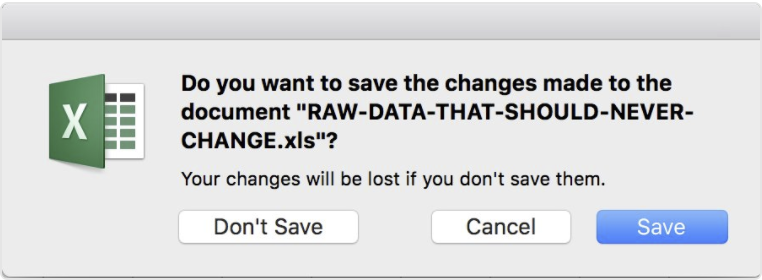
\includegraphics{Figure/dont_overwrite_original.png}

\end{frame}

\begin{frame}[fragile]{Getting data into \textbf{R}}

\begin{itemize}
\item
  Always set a working directory using \texttt{setwd()}, this can be a
  directory where you store the data and/or outputting the results.

  \begin{itemize}
  \tightlist
  \item
    Ignore this if you are using the \textbf{R}studio project.
  \item
    Grey text under the ``Console'' tab.
  \end{itemize}
\item
  Use \texttt{read.csv()} to read a CSV file into \textbf{R}.
\item
  \texttt{dim()}: Returns the number of observations (rows) and
  variables (columns).
\item
  \texttt{head()}/\texttt{tail()}: Returns the first/last 6 rows of a
  data set.
\item
  \texttt{str()}: Returns the structure of the dataset, e.g., dimension,
  column names, type of data object, first few values of each variable.
\item
  \texttt{names()}: Returns the names of the variables contained in a
  dataset.
\end{itemize}

\end{frame}

\begin{frame}[fragile]{CSV file containing patient information}

The patient CSV file has 7 variables:

\begin{itemize}
\tightlist
\item
  \texttt{Patient.ID}: Identification Number.
\item
  \texttt{Age}: in years
\item
  \texttt{Sex}: 0 = Female, 1 = Male
\item
  \texttt{Race}: 1 = Caucasian, 2 = African, 3 = Other
\item
  \texttt{Weight}: in pounds
\item
  \texttt{Height}: in inches
\item
  \texttt{Smoke}: 1 = Yes, 2 = No
\end{itemize}

\end{frame}

\begin{frame}[fragile]{Getting data into \textbf{R}}

\begin{Shaded}
\begin{Highlighting}[]
\CommentTok{# setwd('your working directory')}
\NormalTok{patient.df <-}\StringTok{ }\KeywordTok{read.csv}\NormalTok{(}\StringTok{"Data/Patient.csv"}\NormalTok{)}
\KeywordTok{head}\NormalTok{(patient.df)}
\end{Highlighting}
\end{Shaded}

\begin{verbatim}
##   Patient.ID Age    Sex Race Weight Height Smoke
## 1          3  21   Male    1  179.5   70.4    NA
## 2          4  32 Female    1     NA   63.9    NA
## 3          9  48 Female    1  149.7   61.8     2
## 4         10  35   Male    1  203.5   69.8    NA
## 5         11  48   Male    1  155.3     NA     2
## 6         19  44   Male    2  189.6   70.2     1
\end{verbatim}

\begin{quote}
You can use 1 forwardslash (\texttt{/}) or 2 backslashes
(\texttt{\textbackslash{}\textbackslash{}}).
\end{quote}

\begin{Shaded}
\begin{Highlighting}[]
\CommentTok{# setwd('your working directory')}
\NormalTok{patient.df <-}\StringTok{ }\KeywordTok{read.csv}\NormalTok{(}\StringTok{"Data}\CharTok{\textbackslash{}\textbackslash{}}\StringTok{Patient.csv"}\NormalTok{)}
\end{Highlighting}
\end{Shaded}

\begin{quote}
Tip: use ``Tab'' key to choose to files in \texttt{read.csv()} function,
within the quotation (\texttt{""}).
\end{quote}

\end{frame}

\begin{frame}[fragile]{Check the variable names}

\begin{Shaded}
\begin{Highlighting}[]
\CommentTok{# Names of the variables}
\KeywordTok{names}\NormalTok{(patient.df)}
\NormalTok{## [1] "Patient.ID" "Age"        "Sex"       }
\NormalTok{## [4] "Race"       "Weight"     "Height"    }
\NormalTok{## [7] "Smoke"}
\end{Highlighting}
\end{Shaded}

\begin{itemize}
\tightlist
\item
  Anything following the \texttt{\#} symbol is treated as a comment and
  ignored by \textbf{R}.
\item
  Writing comments/documentation is a very good habit to develop,
  emphasis on \emph{why}.
\end{itemize}

\end{frame}

\begin{frame}[fragile]{\texttt{dim()} and \texttt{str()}}

\begin{Shaded}
\begin{Highlighting}[]
\KeywordTok{dim}\NormalTok{(patient.df)}
\NormalTok{## [1] 200   7}
\KeywordTok{str}\NormalTok{(patient.df)}
\NormalTok{## 'data.frame':    200 obs. of  7 variables:}
\NormalTok{##  $ Patient.ID: int  3 4 9 10 11 19 34 44 45 48 ...}
\NormalTok{##  $ Age       : int  21 32 48 35 48 44 42 24 67 56 ...}
\NormalTok{##  $ Sex       : Factor w/ 2 levels "Female","Male": 2 1 1 2 2 2 1 1 1 1 ...}
\NormalTok{##  $ Race      : int  1 1 1 1 1 2 2 1 2 1 ...}
\NormalTok{##  $ Weight    : num  180 NA 150 204 155 ...}
\NormalTok{##  $ Height    : num  70.4 63.9 61.8 69.8 NA 70.2 62.6 64.4 64.3 67.6 ...}
\NormalTok{##  $ Smoke     : int  NA NA 2 NA 2 1 1 1 NA 2 ...}
\end{Highlighting}
\end{Shaded}

Note that \textbf{character} vector, \texttt{Sex}, is automatically
converted to \textbf{factor}.

\end{frame}

\begin{frame}[fragile]{Reading data into \textbf{R}}

\begin{Shaded}
\begin{Highlighting}[]
\NormalTok{patient.df <-}\StringTok{ }\KeywordTok{read.csv}\NormalTok{(}\StringTok{"Data/Patient.csv"}\NormalTok{, }
                       \DataTypeTok{stringsAsFactors =} \OtherTok{FALSE}\NormalTok{)}
\KeywordTok{str}\NormalTok{(patient.df)}
\end{Highlighting}
\end{Shaded}

\begin{verbatim}
## 'data.frame':    200 obs. of  7 variables:
##  $ Patient.ID: int  3 4 9 10 11 19 34 44 45 48 ...
##  $ Age       : int  21 32 48 35 48 44 42 24 67 56 ...
##  $ Sex       : chr  "Male" "Female" "Female" "Male" ...
##  $ Race      : int  1 1 1 1 1 2 2 1 2 1 ...
##  $ Weight    : num  180 NA 150 204 155 ...
##  $ Height    : num  70.4 63.9 61.8 69.8 NA 70.2 62.6 64.4 64.3 67.6 ...
##  $ Smoke     : int  NA NA 2 NA 2 1 1 1 NA 2 ...
\end{verbatim}

\begin{block}{\texttt{stringsAsFactors}}

\texttt{stringsAsFactors} argument is set to \texttt{FALSE}, so
\textbf{character} vectors are not converted to \textbf{factor} vectors.
We will explain factor in Session 3.

\end{block}

\end{frame}

\begin{frame}[fragile]{Different types of data objects in \textbf{R}}

\textbf{R} has 6 different types of object:

\begin{itemize}
\tightlist
\item
  \texttt{character} (alphanumeric; \texttt{"hello\ world"}), e.g.
  \texttt{Sex}
\item
  \texttt{numeric} (real or decimal; \texttt{3.14159}), e.g.
  \texttt{Weight}, \texttt{Height} and \texttt{Smoke}.
\item
  \texttt{integer} (whole numbers; \texttt{256}), e.g.
  \texttt{Patient.ID}, \texttt{Age}, \texttt{Race}.
\item
  \texttt{logical} (\texttt{TRUE} (\texttt{T}) or \texttt{FALSE}
  (\texttt{F})), e.g.
\end{itemize}

\begin{Shaded}
\begin{Highlighting}[]
\DecValTok{1} \OperatorTok{==}\StringTok{ }\DecValTok{1}
\NormalTok{## [1] TRUE}
\DecValTok{2} \OperatorTok{<=}\StringTok{ }\DecValTok{0}
\NormalTok{## [1] FALSE}
\DecValTok{3} \OperatorTok{!=}\StringTok{ }\DecValTok{2}
\NormalTok{## [1] TRUE}
\end{Highlighting}
\end{Shaded}

\begin{itemize}
\tightlist
\item
  \texttt{factor} (numeric or alphanumeric, treated as categorical)
\item
  \texttt{complex} (numbers with imaginary components; \texttt{3i})
\end{itemize}

\end{frame}

\begin{frame}[fragile]{Vectors}

\begin{itemize}
\tightlist
\item
  Use \texttt{c()} to combine multiple elements separated by comma's.
\item
  A \emph{vector} is a combination of multiple elements of the same
  object type in 1 dimension (a one-dimensional array).
\end{itemize}

\begin{Shaded}
\begin{Highlighting}[]
\CommentTok{# A character vector contains strings}
\KeywordTok{c}\NormalTok{(}\StringTok{"hello"}\NormalTok{, }\StringTok{"world"}\NormalTok{)}
\NormalTok{## [1] "hello" "world"}

\CommentTok{# A numeric vector contains numbers}
\KeywordTok{c}\NormalTok{(}\DecValTok{1}\NormalTok{, }\DecValTok{2}\NormalTok{, }\DecValTok{3}\NormalTok{, }\DecValTok{4}\NormalTok{, }\DecValTok{5}\NormalTok{, }\DecValTok{6}\NormalTok{)}
\NormalTok{## [1] 1 2 3 4 5 6}

\CommentTok{# We can easily produce sequences using ':'}
\DecValTok{1}\OperatorTok{:}\DecValTok{6}
\NormalTok{## [1] 1 2 3 4 5 6}
\end{Highlighting}
\end{Shaded}

\end{frame}

\begin{frame}[fragile]{Matrices}

\begin{itemize}
\tightlist
\item
  Use \texttt{matrix()} to create a matrix in \textbf{R}.
\item
  A \emph{matrix} is a combination of multiple elements of the same data
  type in 2 dimensions (a 2-dimensional array).
\end{itemize}

\begin{Shaded}
\begin{Highlighting}[]
\CommentTok{# Create a matrix with 2 rows}
\KeywordTok{matrix}\NormalTok{(}\DecValTok{1}\OperatorTok{:}\DecValTok{6}\NormalTok{, }\DataTypeTok{nrow =} \DecValTok{2}\NormalTok{)}
\NormalTok{##      [,1] [,2] [,3]}
\NormalTok{## [1,]    1    3    5}
\NormalTok{## [2,]    2    4    6}

\CommentTok{# Create a matrix with 2 columns}
\KeywordTok{matrix}\NormalTok{(}\DecValTok{1}\OperatorTok{:}\DecValTok{6}\NormalTok{, }\DataTypeTok{ncol =} \DecValTok{2}\NormalTok{)}
\NormalTok{##      [,1] [,2]}
\NormalTok{## [1,]    1    4}
\NormalTok{## [2,]    2    5}
\NormalTok{## [3,]    3    6}
\end{Highlighting}
\end{Shaded}

\end{frame}

\begin{frame}[fragile]{Data frames}

\begin{itemize}
\tightlist
\item
  Use \texttt{data.frame} to create a data frame in \textbf{R}.
\item
  A \emph{data frame} is a collection of multiple vectors (as different
  columns) that can be different types.
\end{itemize}

\begin{Shaded}
\begin{Highlighting}[]
\NormalTok{my_characters =}\StringTok{ }\KeywordTok{c}\NormalTok{(}\StringTok{"one"}\NormalTok{, }\StringTok{"two"}\NormalTok{, }\StringTok{"three"}\NormalTok{)}
\NormalTok{my_numbers =}\StringTok{ }\DecValTok{1}\OperatorTok{:}\DecValTok{3}
\NormalTok{my_logicals =}\StringTok{ }\KeywordTok{c}\NormalTok{(}\OtherTok{TRUE}\NormalTok{, }\OtherTok{FALSE}\NormalTok{, F)}

\KeywordTok{data.frame}\NormalTok{(my_characters, my_numbers, my_logicals)}
\NormalTok{##   my_characters my_numbers my_logicals}
\NormalTok{## 1           one          1        TRUE}
\NormalTok{## 2           two          2       FALSE}
\NormalTok{## 3         three          3       FALSE}
\end{Highlighting}
\end{Shaded}

\end{frame}

\begin{frame}{General Tips (Hotkeys)}

\begin{longtable}[]{@{}ll@{}}
\toprule
Hotkeys & Description\tabularnewline
\midrule
\endhead
Ctrl+Enter & Run Selected Line(s) of code in the Source
pane\tabularnewline
Ctrl+Shift+A & Tidy Selected Line(s) of code in the Source
pane\tabularnewline
Ctrl+Shift+C & Comment Selected Line(s) of code in the Source
pane\tabularnewline
Tab & Complete code in Source or Console pane\tabularnewline
Ctrl+l & Clean the screen the to Console pane\tabularnewline
Esc & Kill the current operation\tabularnewline
Ctrl+Shift+F10 & Restart \textbf{R} (Unload all the loaded \textbf{R}
packages)\tabularnewline
Ctrl+Up & Popup History\tabularnewline
Alt+Shift+K & Show all Hot keys\tabularnewline
\bottomrule
\end{longtable}

\end{frame}

\begin{frame}{Common Mistakes}

\begin{itemize}
\tightlist
\item
  Spelling, inculding the upper/lower cases.
\item
  Matching parentheses/brackets and quotation symbols.
\end{itemize}

\end{frame}

\begin{frame}{Summary}

\begin{itemize}
\tightlist
\item
  Quick introduction to \textbf{R} and RStudio
\item
  Spreadsheet guidelines
\item
  Getting data into \textbf{R}
\end{itemize}

\end{frame}

\end{document}
